% Copyright (c) 2015 William Bevington, Callum O'Brien and Alex Pace

% Permission is granted to copy, distribute and/or modify this document
% under the terms of the GNU Free Documentation License, Version 1.3
% or any later version published by the Free Software Foundation;
% with no Invariant Sections, no Front-Cover Texts, and no Back-Cover Texts.

\documentclass{article}

\usepackage{amsmath}
\usepackage{amssymb}

\usepackage{array}

\usepackage{geometry}

\usepackage{mathrsfs}

\usepackage{multicol}

\usepackage{tikz}
\usetikzlibrary{arrows}

\newcommand{\csch}{\textrm{cosech\:}}
\newcommand{\sech}{\textrm{sech\:}}

\title{FP3}
\author{William Bevington \and Callum O'Brien \and Alex Pace}

\begin{document}

\maketitle
\tableofcontents
\newpage

\section{Hyperbolic Functions}

\subsection{Hyperbolic Sine \& Cosecant}

\begin{center}

    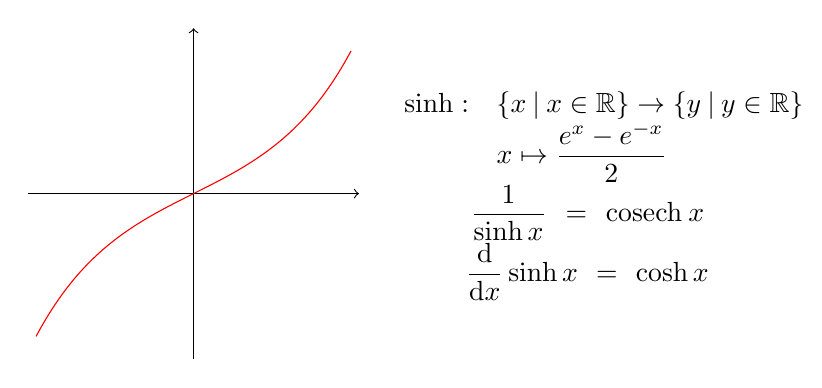
\begin{tikzpicture}

        \draw [->] (-2.1,0) -- (2.1,0);
        \draw [->] (0,-2.1) -- (0,2.1);
        \draw [red, domain=-2:2, samples=100] plot (\x, {0.5 * sinh \x});

        \draw (5,0) node [text width=5cm, text centered] {
                
            \(\begin{array}{*1{>{\displaystyle}r}{>{\displaystyle}l}}

                \sinh: & \left\{x\:|\:x\in\mathbb{R}\right\}\rightarrow\left\{y\:|\:y\in\mathbb{R}\right\} \\
                & x \mapsto \frac{e^x-e^{-x}}{2} \\

            \end{array}\)\\

            \(\displaystyle\frac{1}{\sinh x}=\csch x\)\\

            \(\displaystyle\frac{\textrm{d}}{\textrm{d}x}\sinh x=\cosh x\)

        };

    \end{tikzpicture}
    
\end{center}

\subsection{Hyperbolic Cosine \& Secant}

\begin{center}

    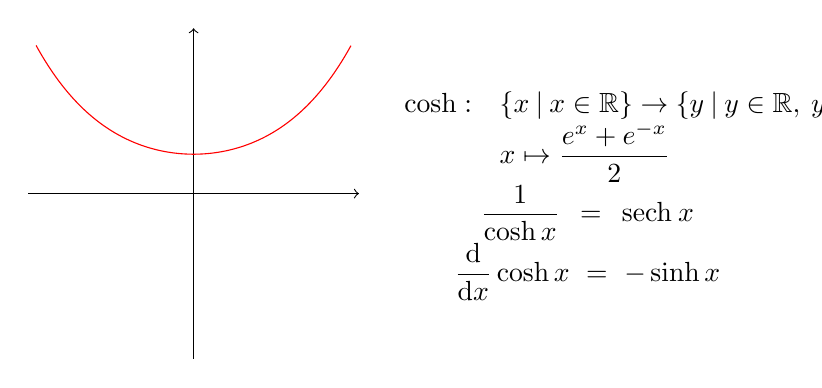
\begin{tikzpicture}
    
        \draw [->] (-2.1,0) -- (2.1,0);
        \draw [->] (0,-2.1) -- (0,2.1);
        \draw [red, domain=-2:2, samples=100] plot (\x, {0.5 * cosh \x});
    
        \draw (5,0) node [text width=5cm, text centered] {
            
            \(\begin{array}{*1{>{\displaystyle}r}{>{\displaystyle}l}}

                \cosh: & \left\{x\:|\:x\in\mathbb{R}\right\}\rightarrow\left\{y\:|\:y\in\mathbb{R},\:y\geq1\right\} \\
                & x \mapsto \frac{e^x+e^{-x}}{2} \\

            \end{array}\)
    
            \(\displaystyle\frac{1}{\cosh x}=\sech x\)

            \(\displaystyle\frac{\textrm{d}}{\textrm{d}x}\cosh x=-\sinh x\)

        };
    
    \end{tikzpicture}

\end{center}

\subsection{Hyperbolic Tangent \& Cotangent}

\begin{center}

    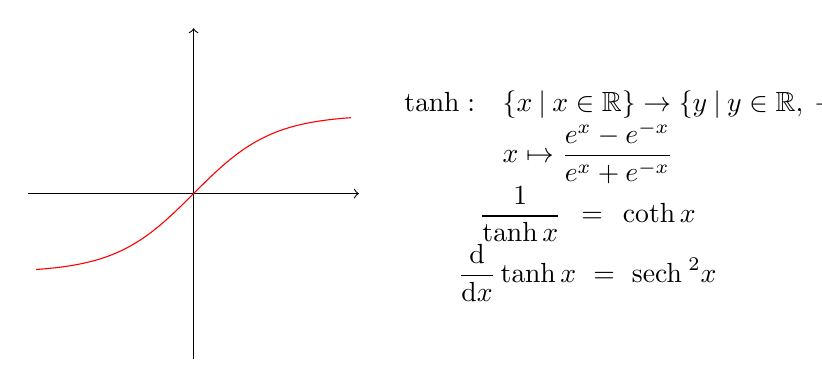
\begin{tikzpicture}

        \draw [->] (-2.1,0) -- (2.1,0);
        \draw [->] (0,-2.1) -- (0,2.1);
        \draw [red, domain=-2:2, samples=100] plot (\x, {tanh \x});
        \draw (5,0) node [text width=5cm, text centered] {
            
            \(\begin{array}{*1{>{\displaystyle}r}{>{\displaystyle}l}}

                \tanh: & \left\{x\:|\:x\in\mathbb{R}\right\}\rightarrow\left\{y\:|\:y\in\mathbb{R},\:-1<y<1\right\} \\
                & x \mapsto \frac{e^x-e^{-x}}{e^x+e^{-x}} \\

            \end{array}\)

            \(\displaystyle\frac{1}{\tanh x}=\coth x\)

            \(\displaystyle\frac{\textrm{d}}{\textrm{d}x}\tanh x=\sech^2 x\)

        };

    \end{tikzpicture}

\end{center}

\end{document}

